% Chapter 4
\chapter{Results \& Discussion} % Main chapter title
The CA model was created and run for 50 generations or time steps. An image was generated of the simulated Building Based Land Usage growth and it was saved. The accuracy of the simulated growth was also calculated and saved. The metric involved for calculating the accuracy  was the Kappa coefficient (Also known as the Cohen's Kappa coefficient)
\begin{center}
$\kappa = (p_o - p_e) / (1 - p_e)$\\
or\\
$\kappa = \frac{(p_o - p_e)}{(1 - p_e)}$
\end{center}
$p_o$ is 

\begin{table}[H]
\centering
\caption{Interpreting the Kappa coefficient magnitude}
\label{table:kap}
\begin{tabular}{@{}ll@{}}
\toprule
\multicolumn{1}{c}{Values} & \multicolumn{1}{c}{Magnitude guideline} \\ \midrule
$\kappa \leq 0$                & No agreement                            \\
$0 \leq \kappa \leq 0.20$                     & Slight agreement                        \\
$0.21 \leq \kappa \leq 0.40$                  & Fair agreement                          \\
$0.41 \leq \kappa \leq 0.60$                  & Moderate agreement                      \\
$0.61 \leq \kappa \leq 0.804$                  & Substantial agreement                   \\
$0.81 \leq \kappa \leq 1$                     & Almost perfect agreement                \\ \bottomrule
\end{tabular}
\end{table}
\label{Chapter4} % For referencing the chapter elsewhere, use \ref{Chapter4}
\begin{figure}[H]
\begin{subfigure}{.5\textwidth}
  \centering
  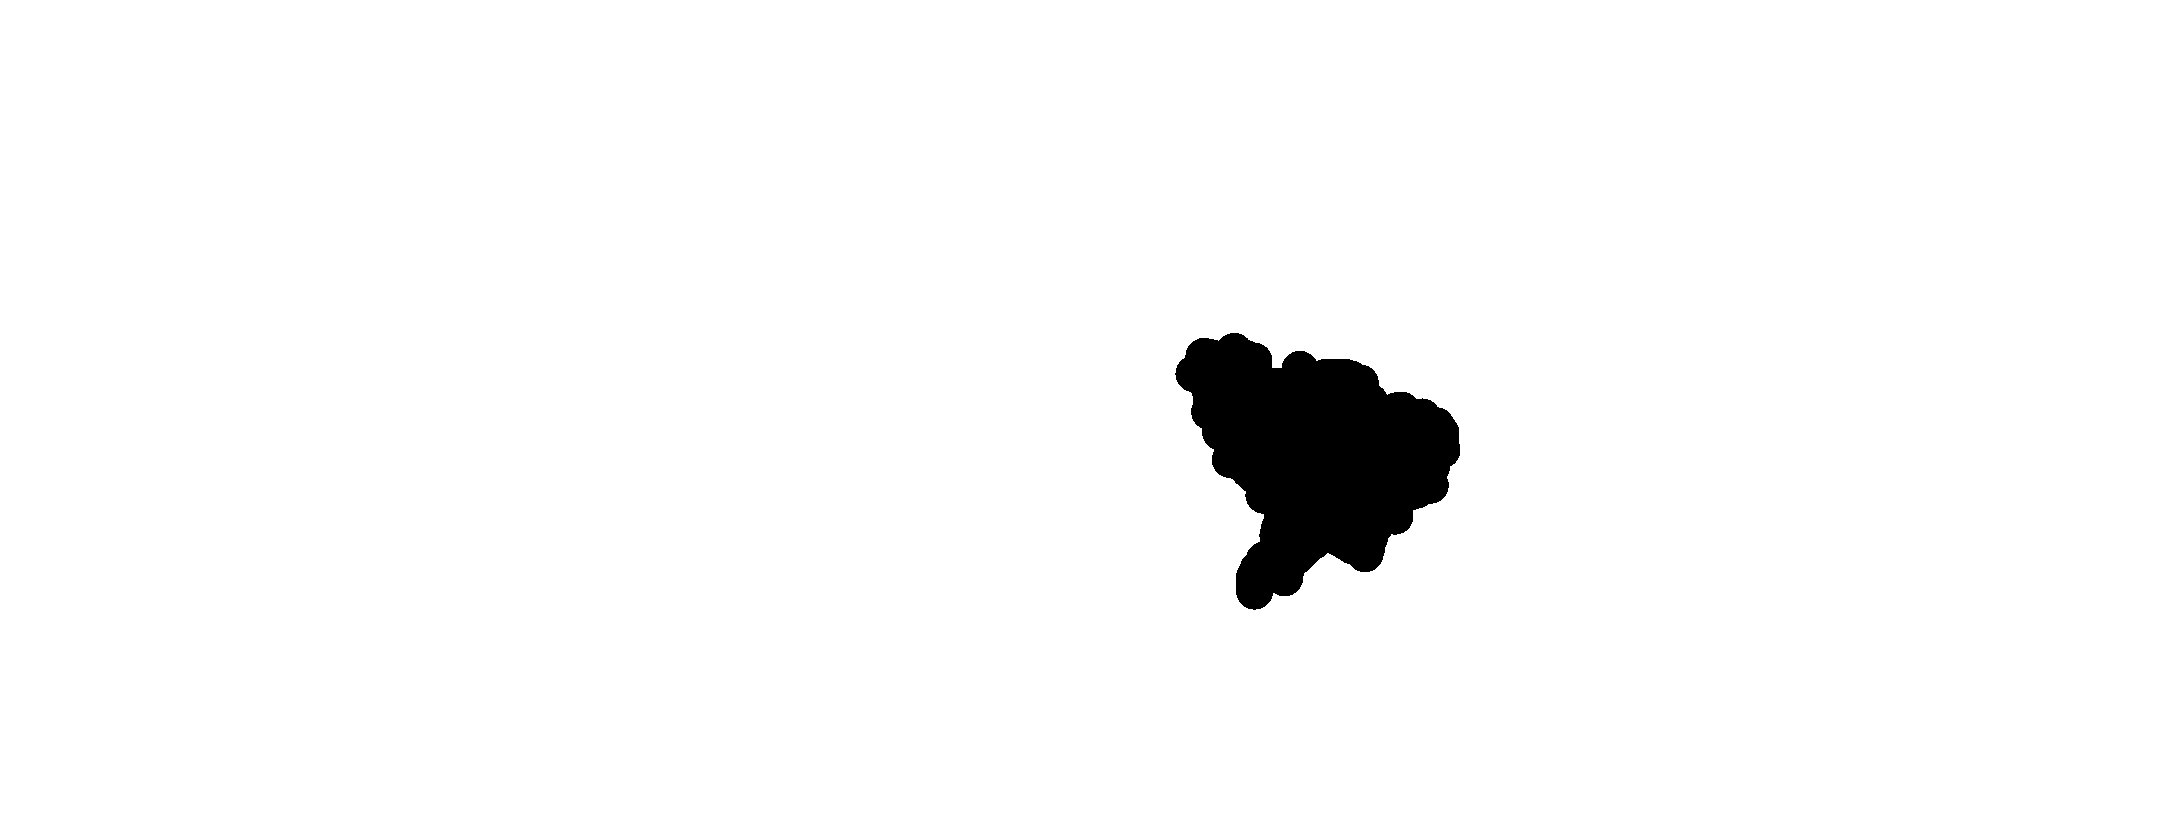
\includegraphics[width=1\linewidth]{Figures/Chapter4/generation-0-melusi}
  \caption*{Initial State}
\end{subfigure}
\begin{subfigure}{.5\textwidth}
  \centering
  
\includegraphics[width=1\linewidth]{Figures/Chapter4/generation-1-melusi}
  \caption*{Generation $t = 1$}
\end{subfigure}
\end{figure}

\begin{figure}[H]
\begin{subfigure}{.5\textwidth}
  \centering
  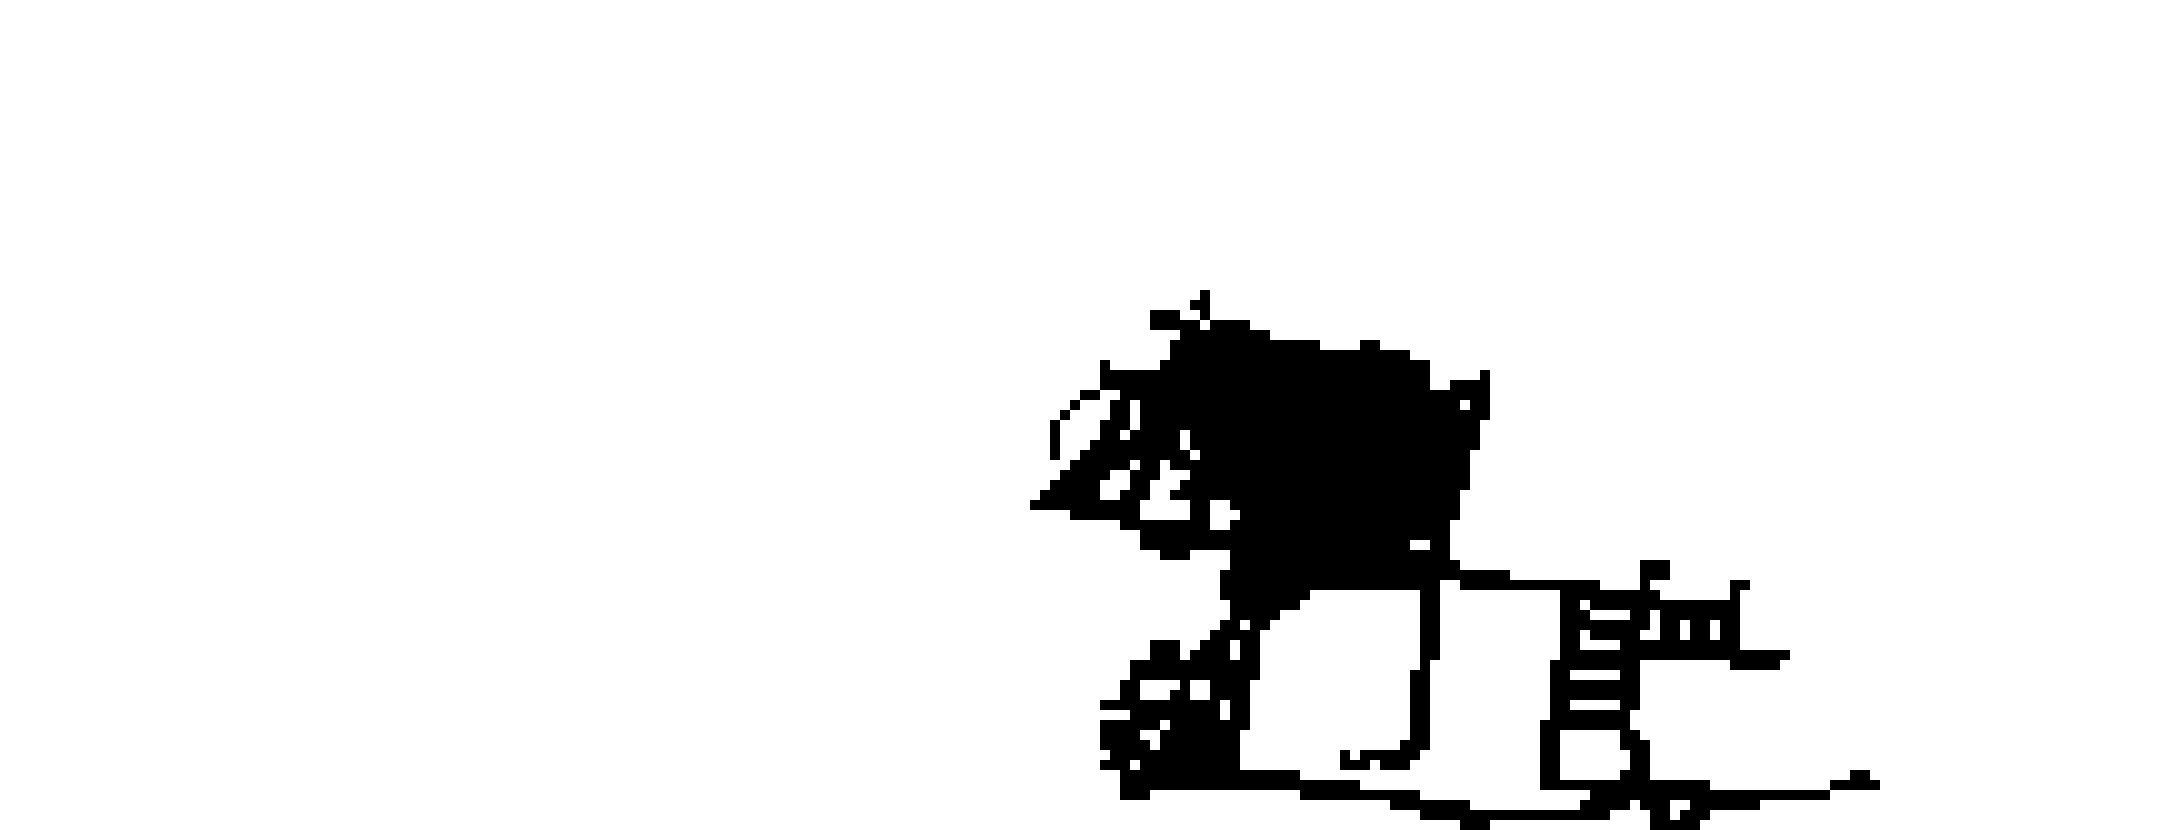
\includegraphics[width=1\linewidth]{Figures/Chapter4/generation-5-melusi}
  \caption*{Generation $t = 5$}
\end{subfigure}
\begin{subfigure}{.5\textwidth}
  \centering
  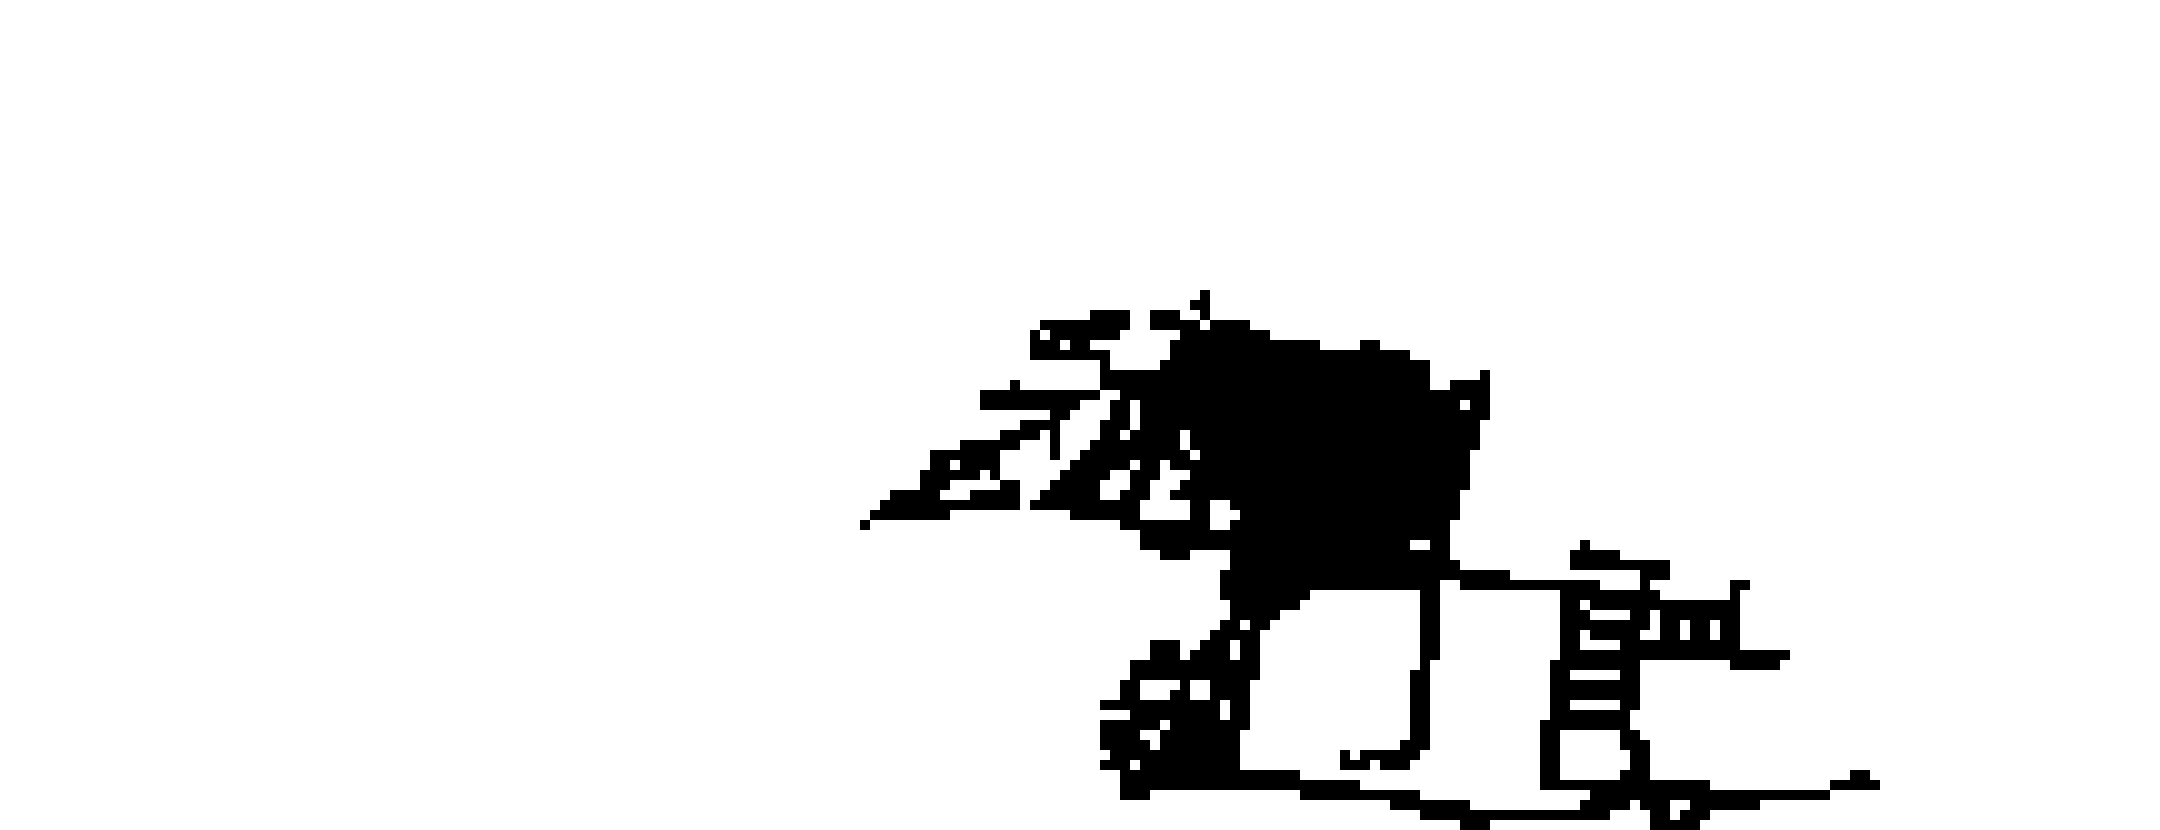
\includegraphics[width=1\linewidth]{Figures/Chapter4/generation-10-melusi}
  \caption*{Generation $t = 10$}
\end{subfigure}
\end{figure}

\begin{figure}[H]
\begin{subfigure}{.5\textwidth}
  \centering
  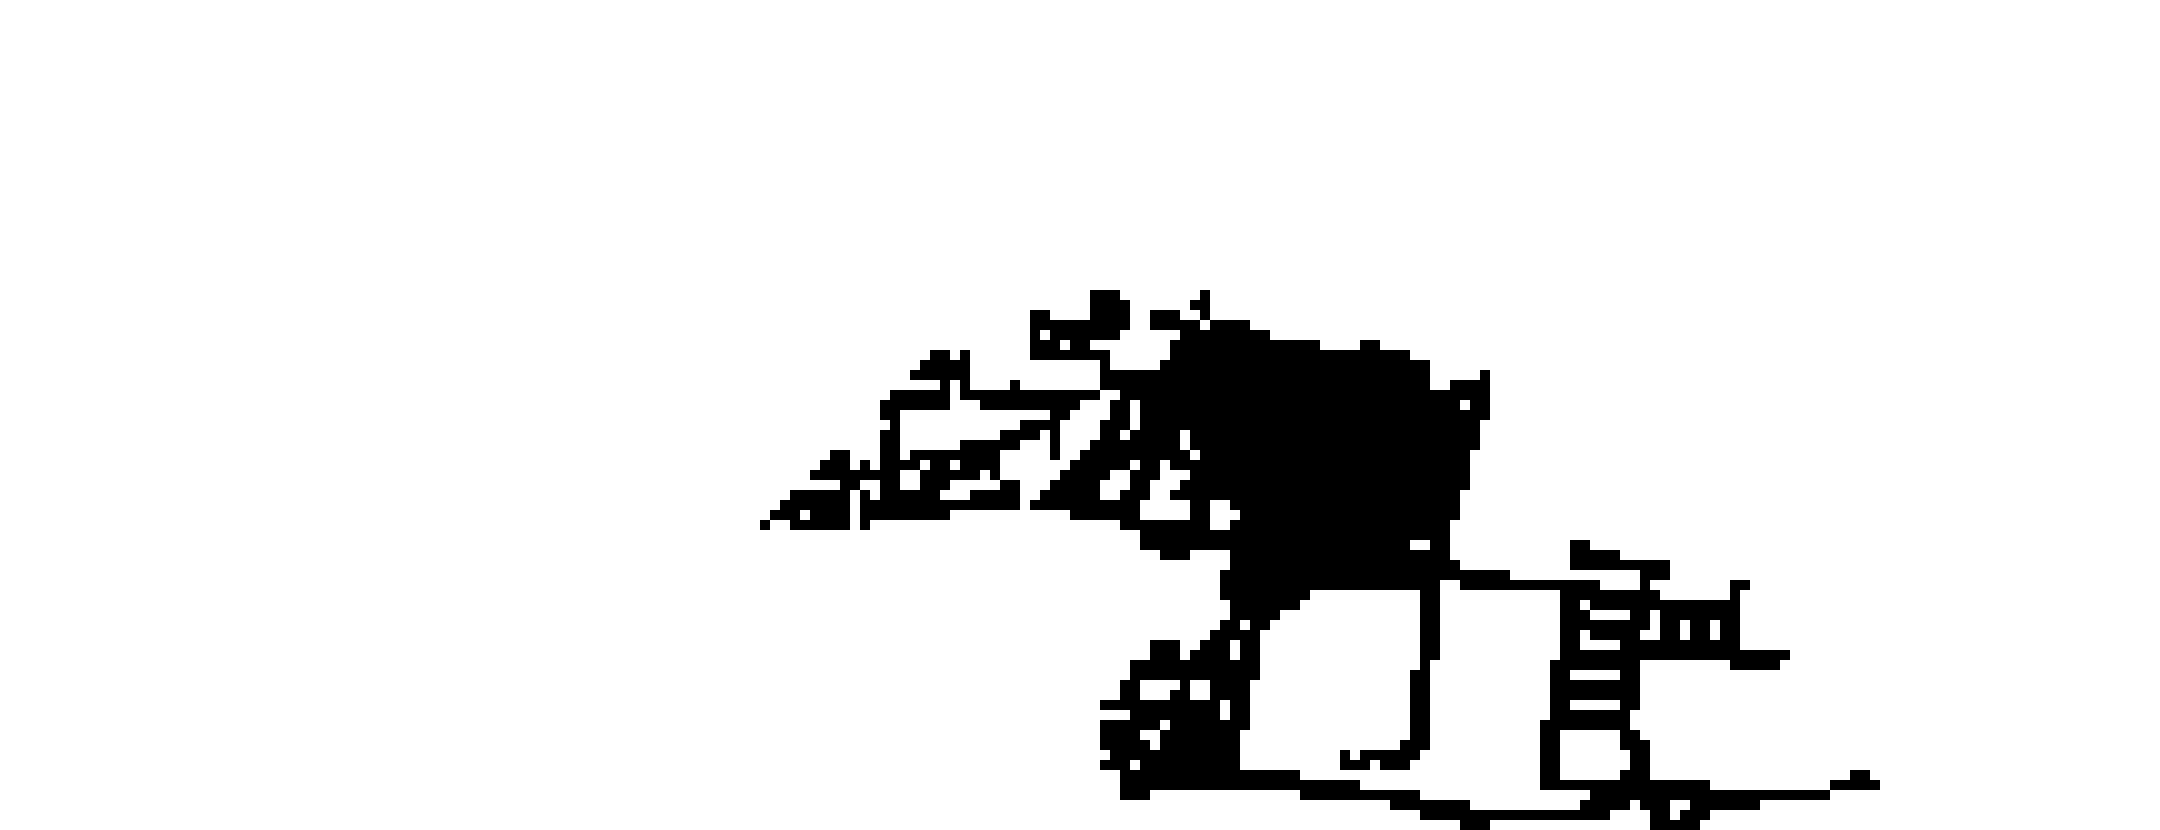
\includegraphics[width=1\linewidth]{Figures/Chapter4/generation-15-melusi}
  \caption*{Generation $t = 15$}
\end{subfigure}
\begin{subfigure}{.5\textwidth}
  \centering
  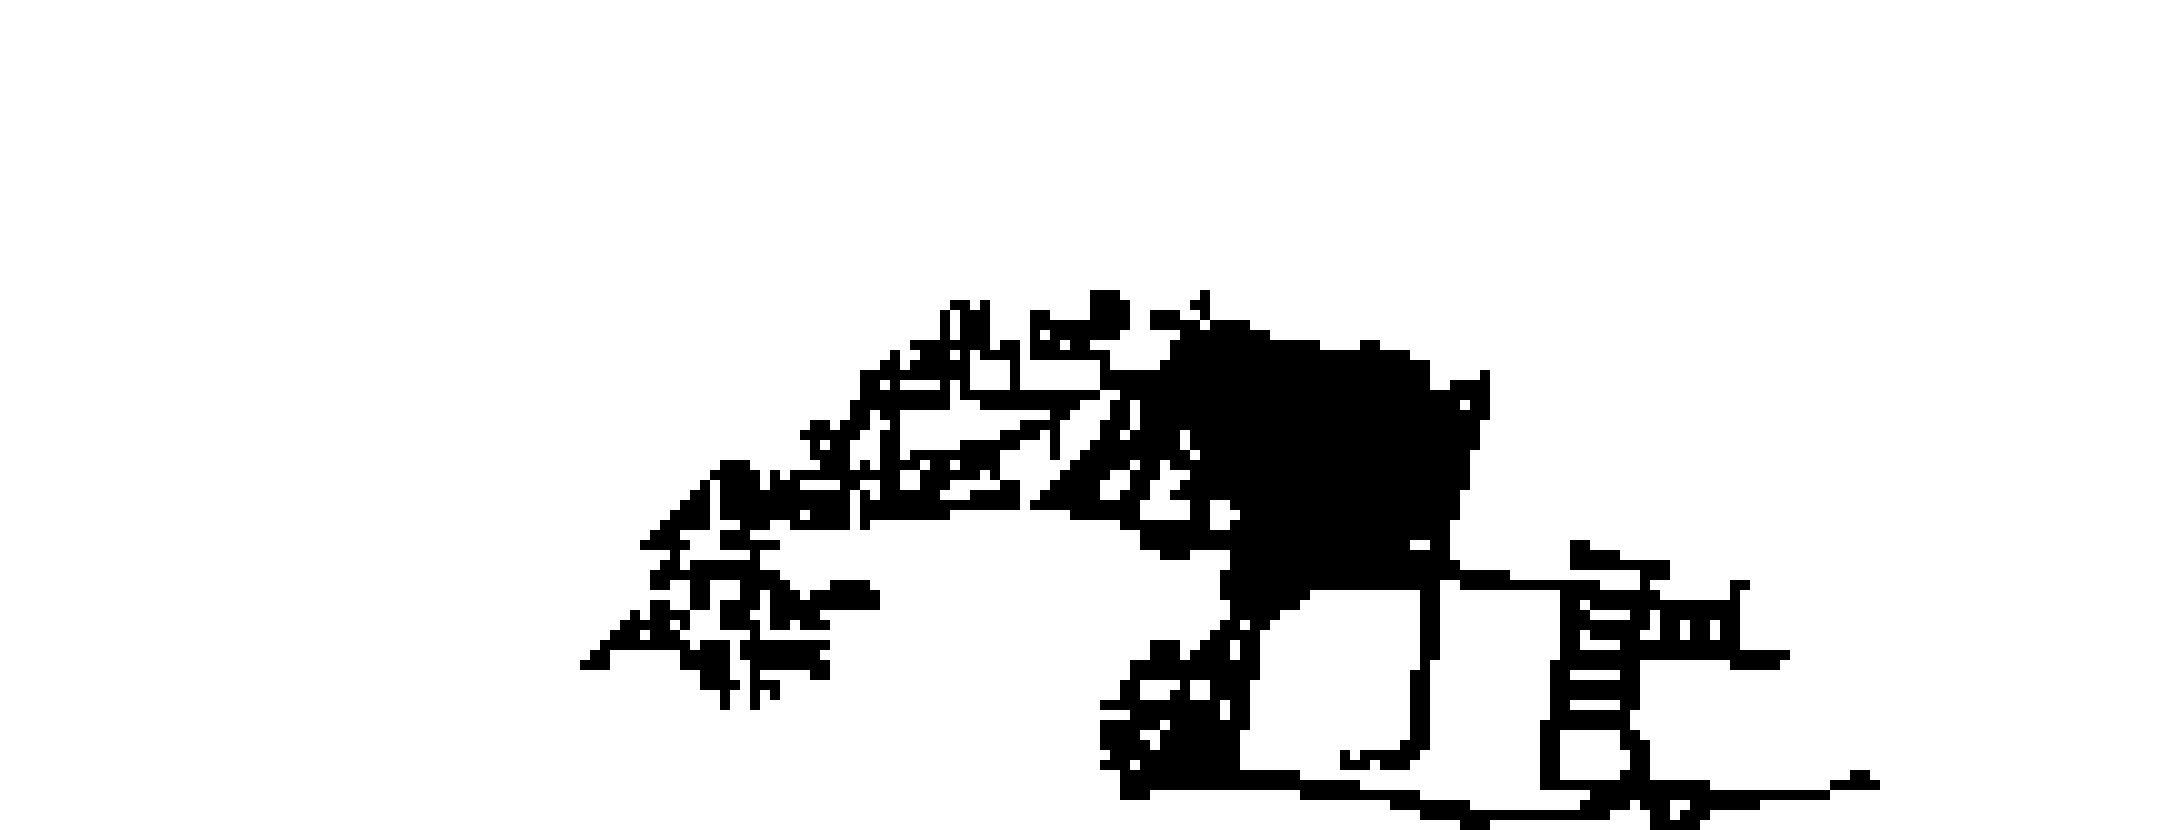
\includegraphics[width=1\linewidth]{Figures/Chapter4/generation-20-melusi}
  \caption*{Generation $t = 20$}
\end{subfigure}
\end{figure}

\begin{figure}[H]
\begin{subfigure}{.5\textwidth}
  \centering
  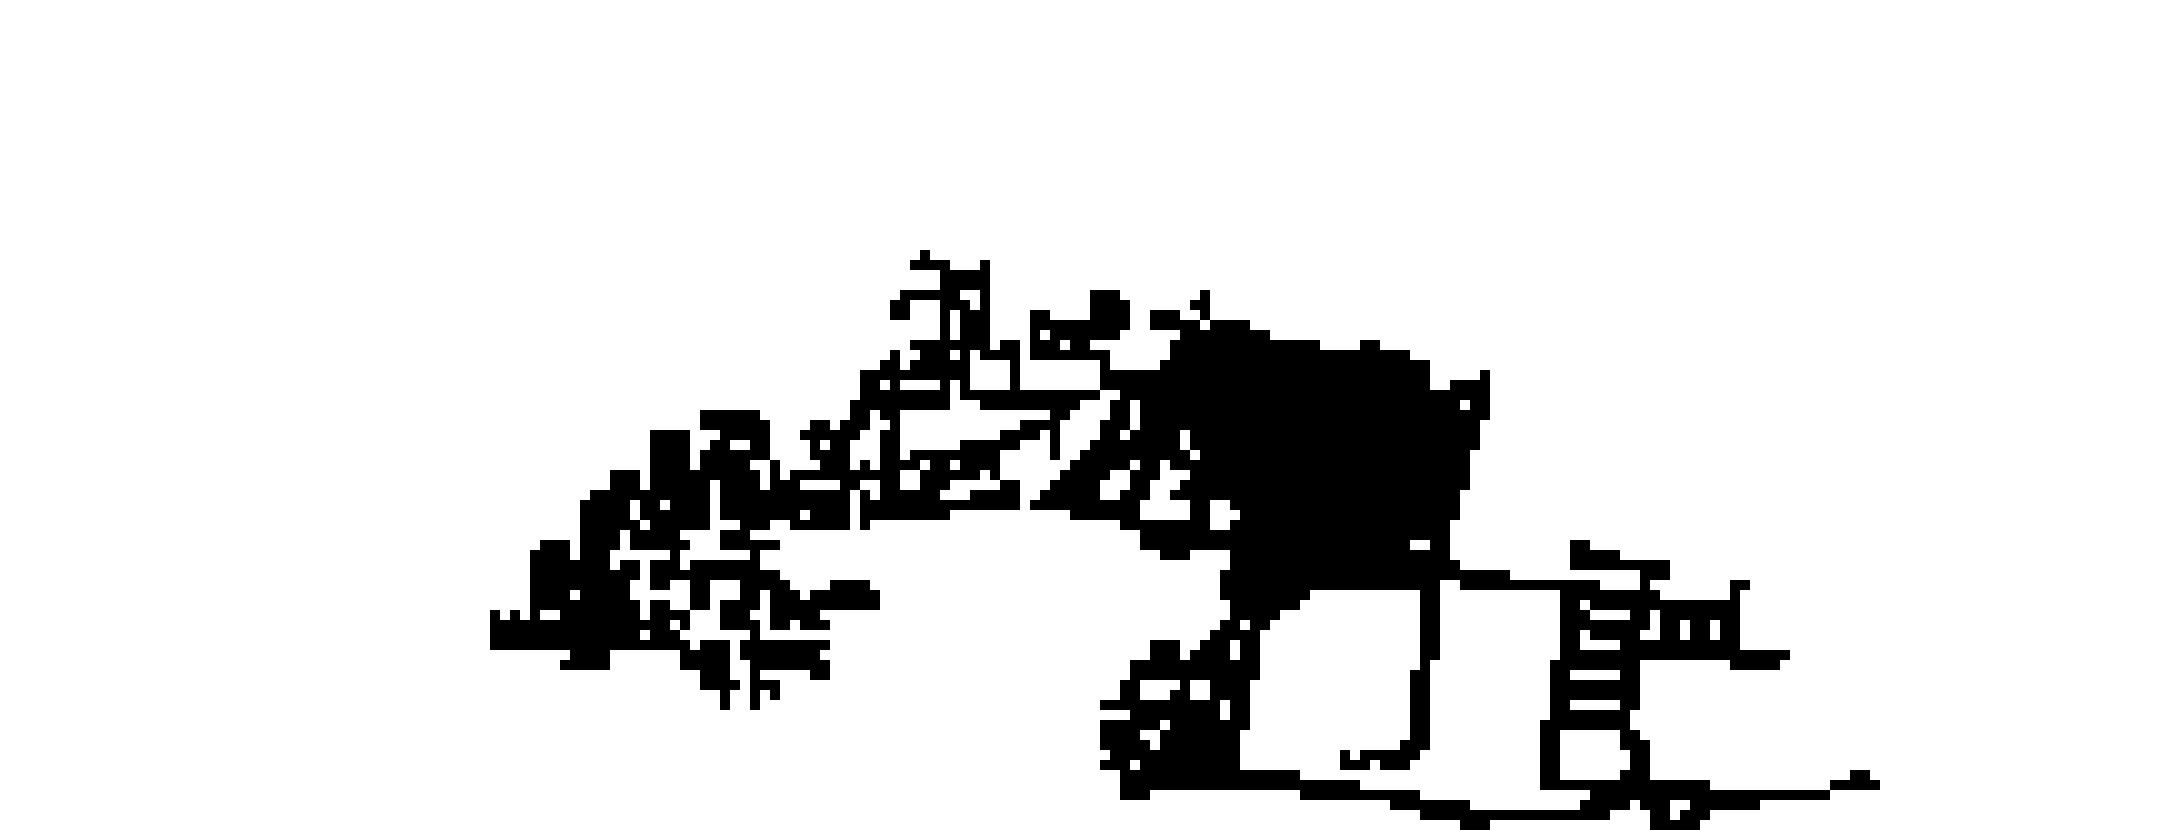
\includegraphics[width=1\linewidth]{Figures/Chapter4/generation-25-melusi}
  \caption*{Generation $t = 25$}
\end{subfigure}
\begin{subfigure}{.5\textwidth}
  \centering
  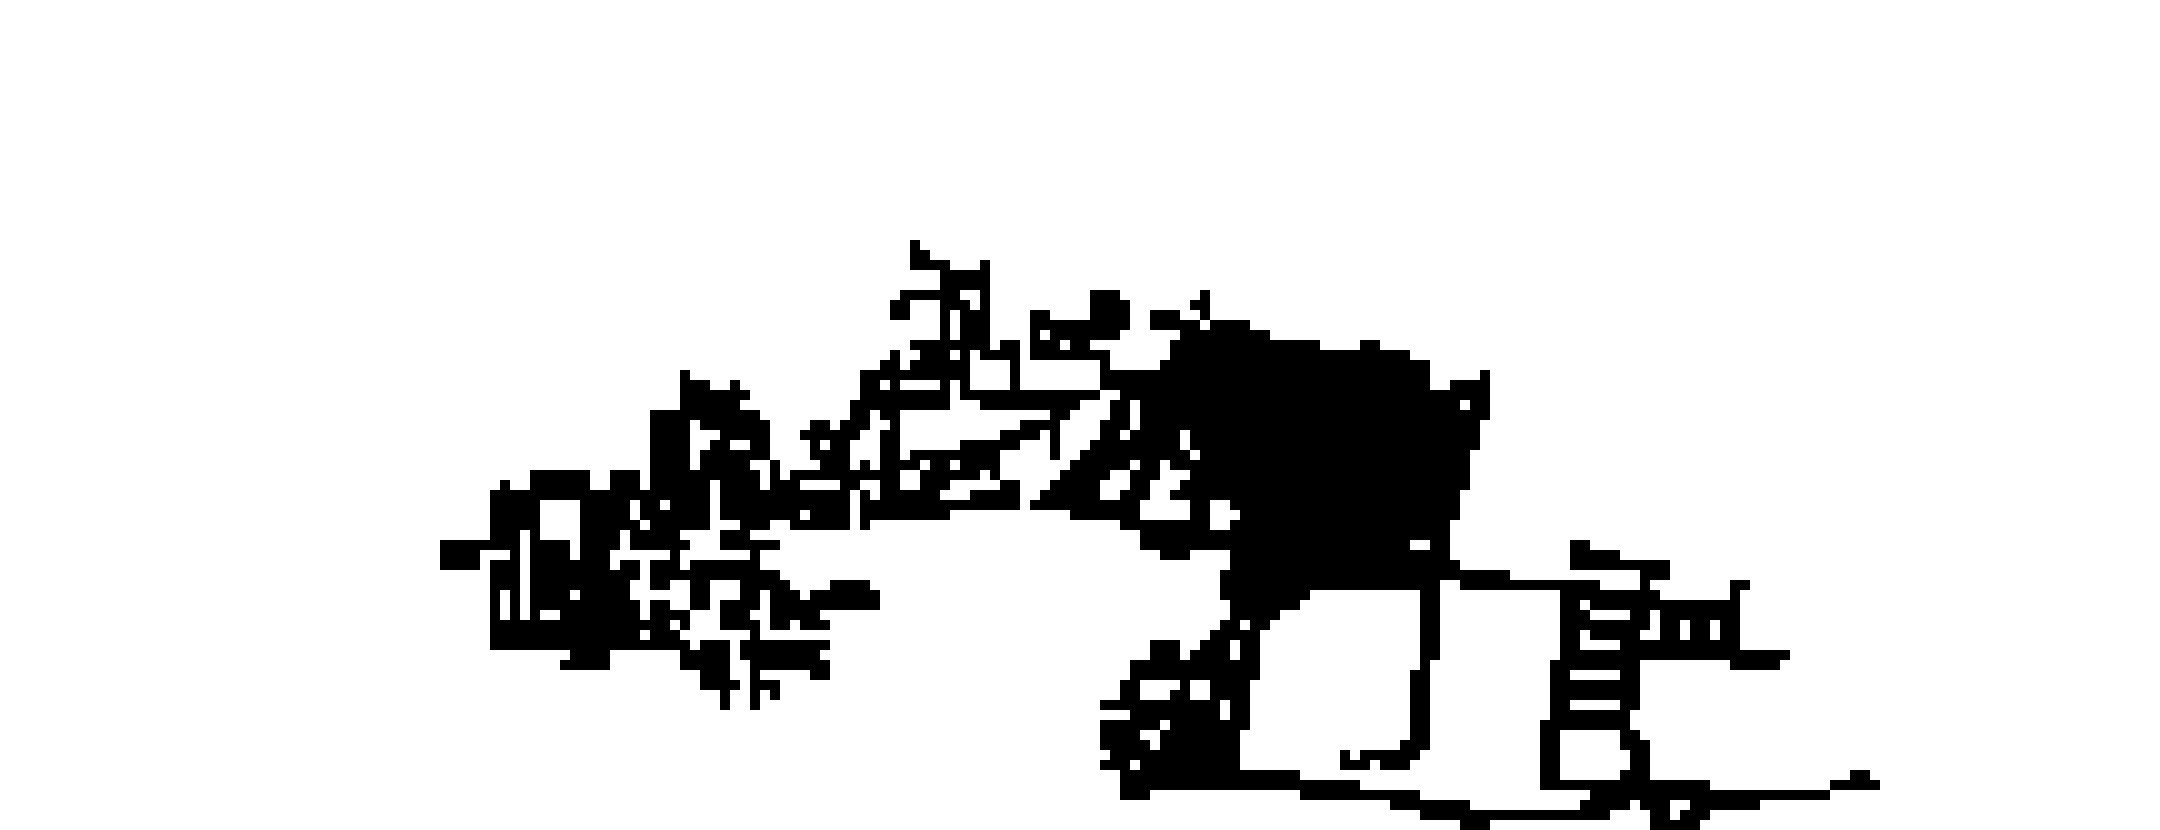
\includegraphics[width=1\linewidth]{Figures/Chapter4/generation-30-melusi}
  \caption*{Generation $t = 30$}
\end{subfigure}
\end{figure}

\begin{figure}[H]
\begin{subfigure}{.5\textwidth}
  \centering
  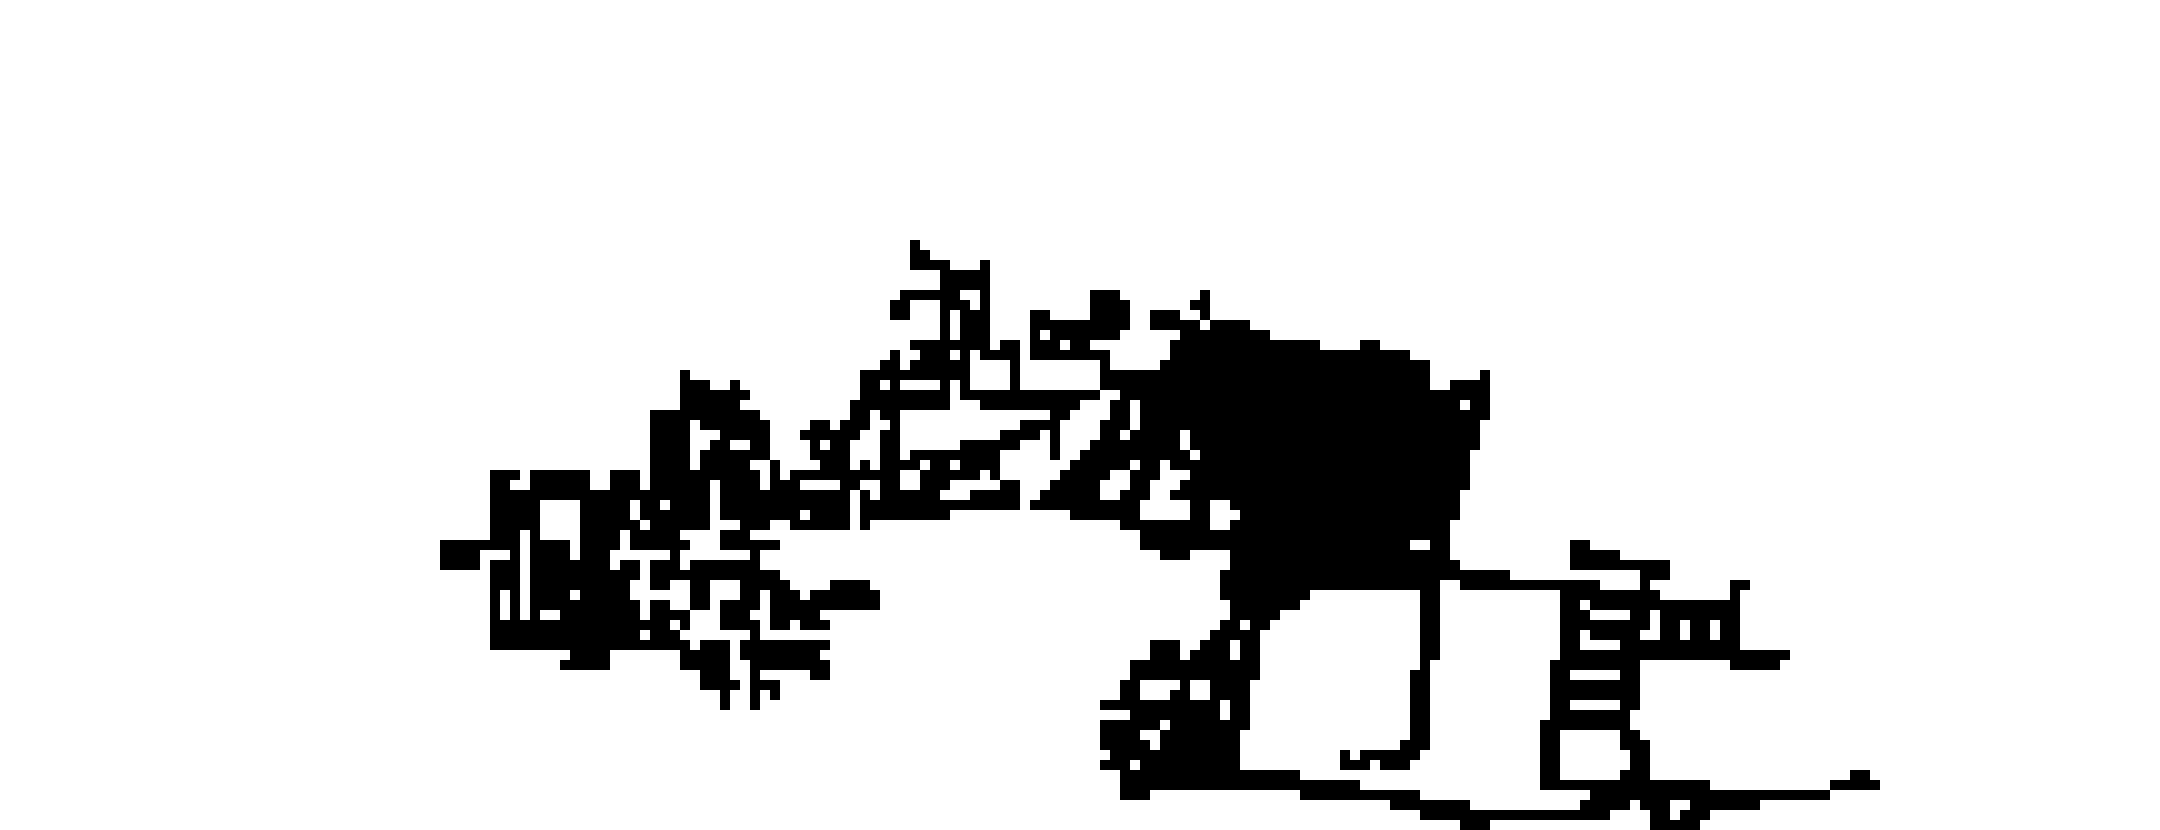
\includegraphics[width=1\linewidth]{Figures/Chapter4/generation-35-melusi}
  \caption*{Generation $t = 35$}
\end{subfigure}
\begin{subfigure}{.5\textwidth}
  \centering
  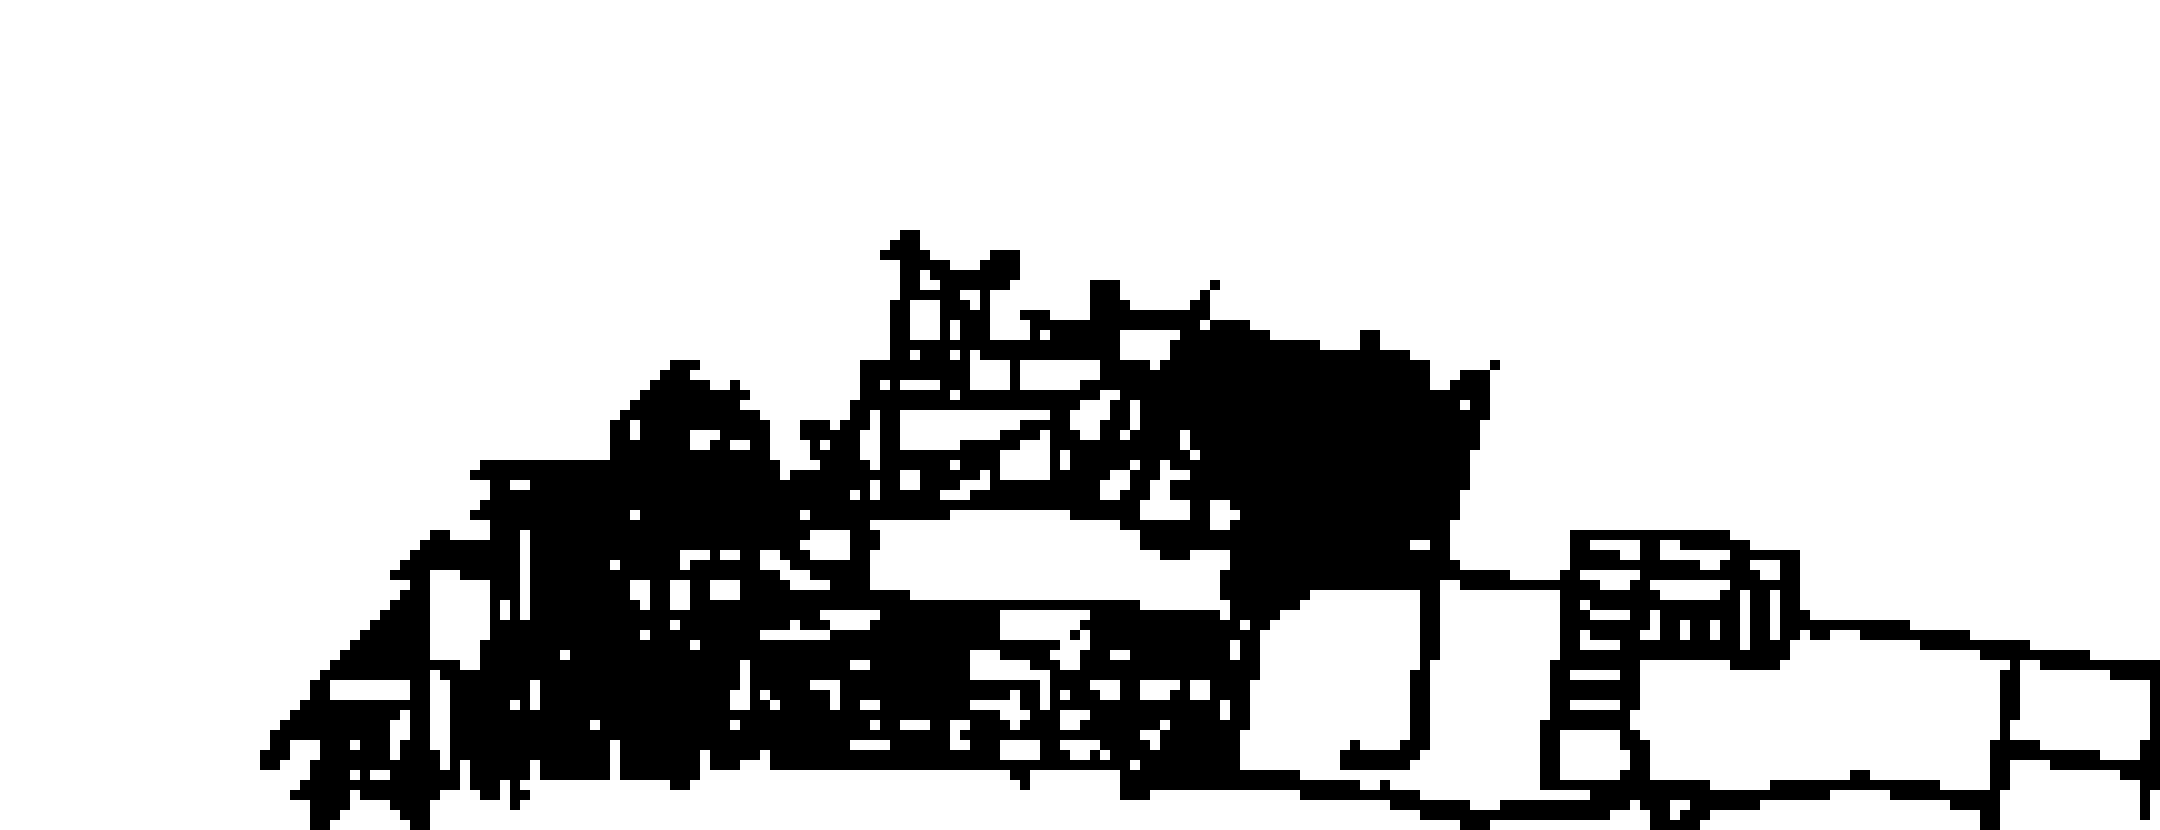
\includegraphics[width=1\linewidth]{Figures/Chapter4/generation-40-melusi}
  \caption*{Generation $t = 40$}
\end{subfigure}
\end{figure}

\begin{figure}[H]
\begin{subfigure}{.5\textwidth}
  \centering
  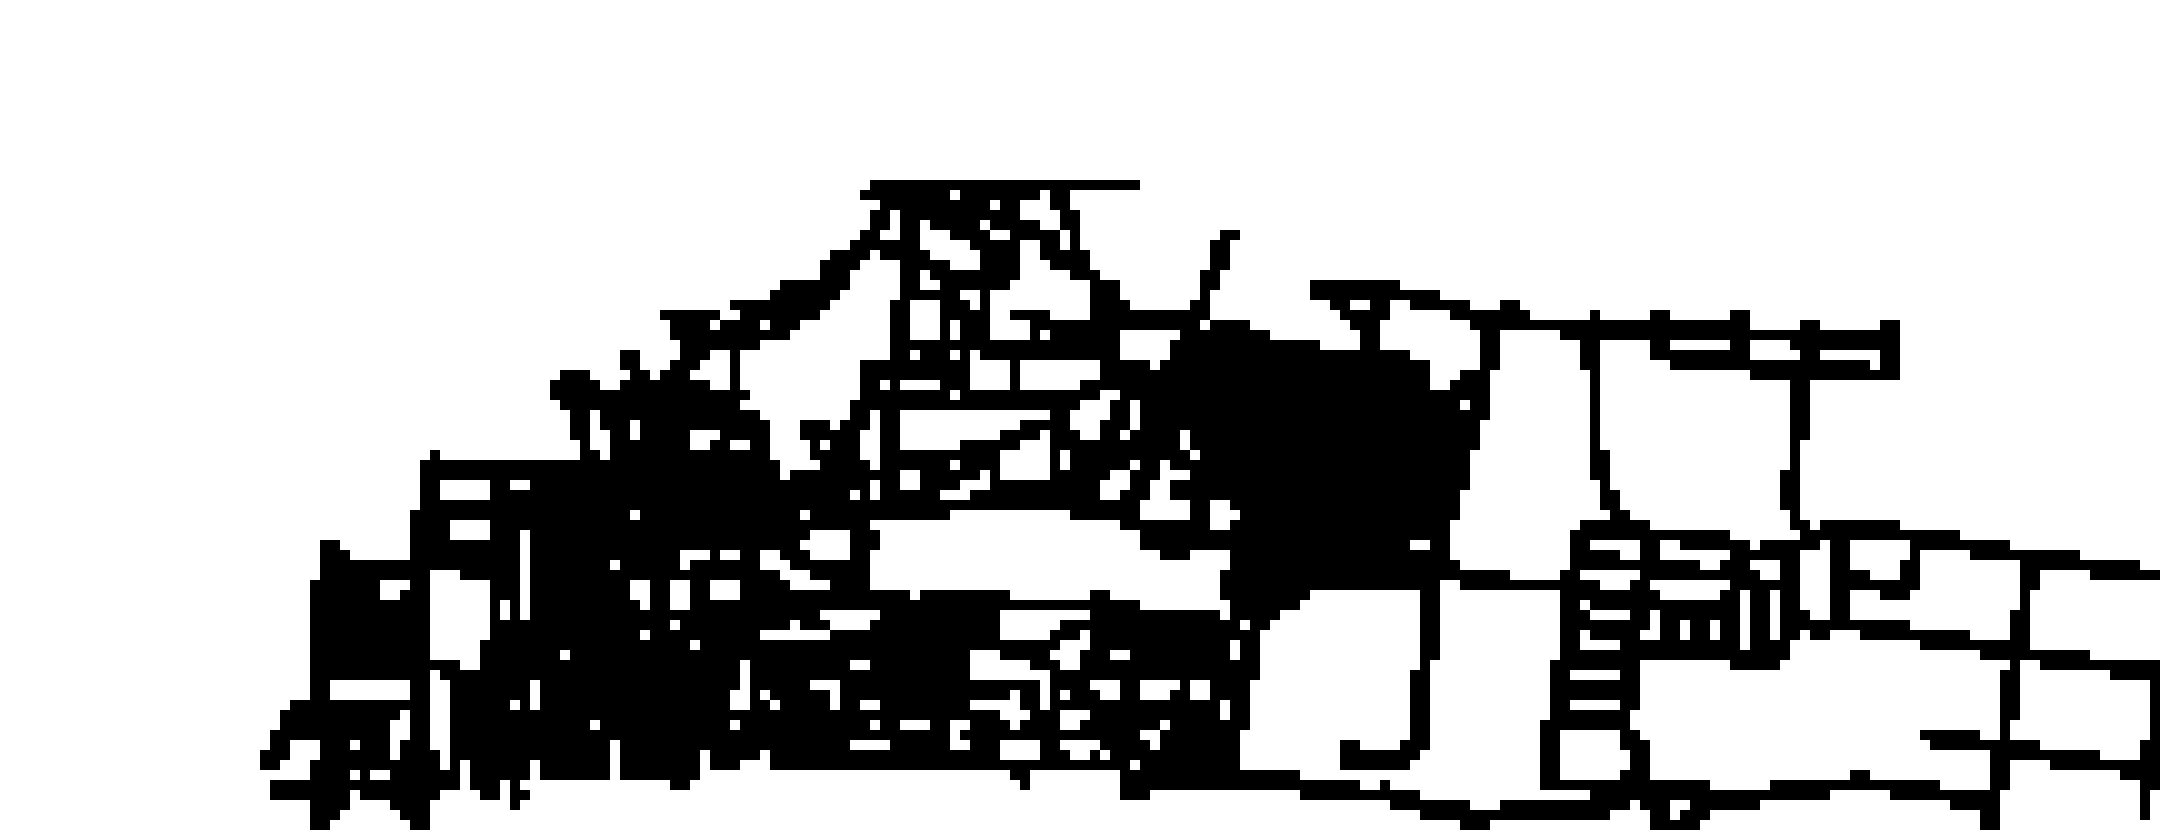
\includegraphics[width=1\linewidth]{Figures/Chapter4/generation-45-melusi}
  \caption{Generation $t = 45$}
\end{subfigure}
\begin{subfigure}{.5\textwidth}
  \centering
  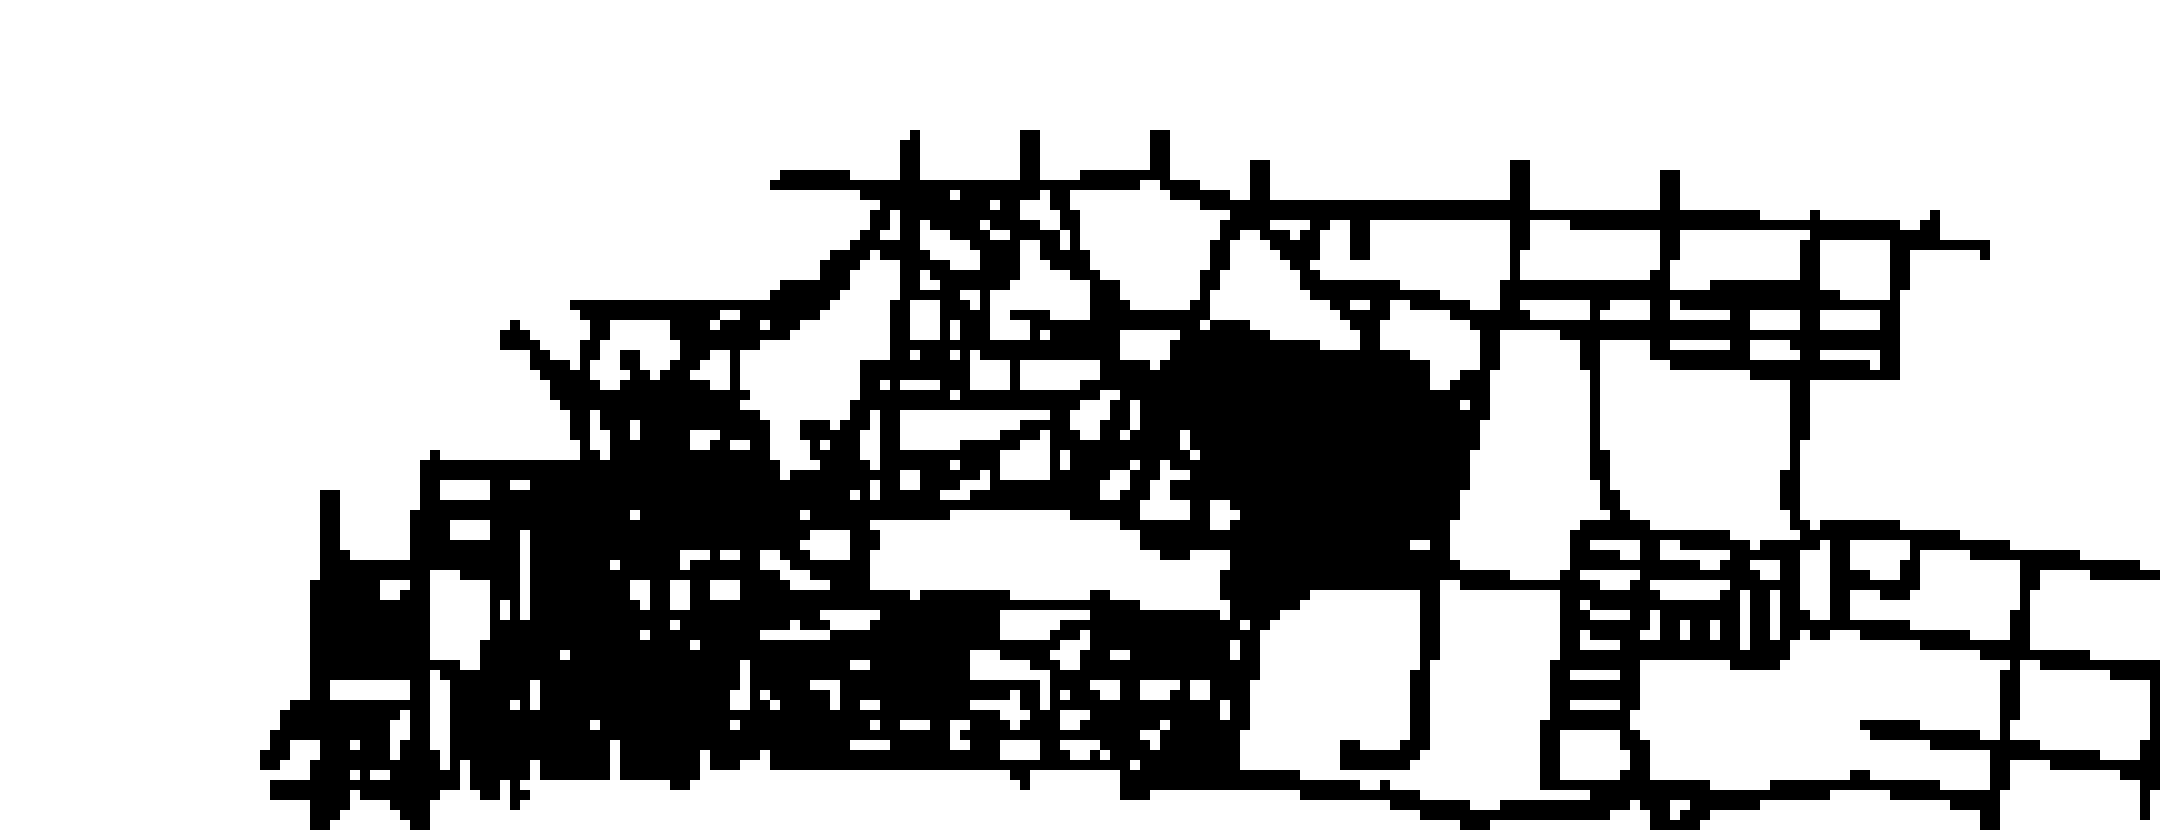
\includegraphics[width=1\linewidth]{Figures/Chapter4/generation-50-melusi}
  \caption{Generation $t = 50$}
\end{subfigure}
\caption{Simulated Growth for different periods of the 50 Generations}
\label{fig:gen50}
\end{figure}
\begin{center}
Source: Own Creation (2021)
\end{center}

\begin{figure}[H]
\centering
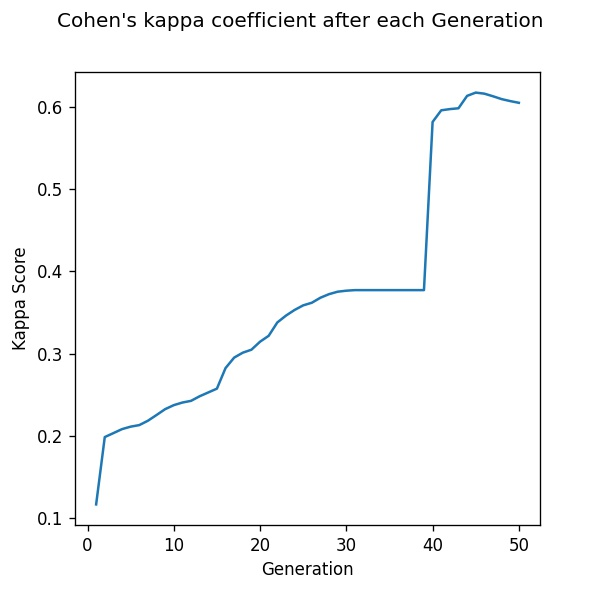
\includegraphics[scale=0.7]{Figures/Chapter4/scoresFigure}
\caption{Kappa coefficient for each generation simulated}
\end{figure}

\begin{figure}[H]
\centering
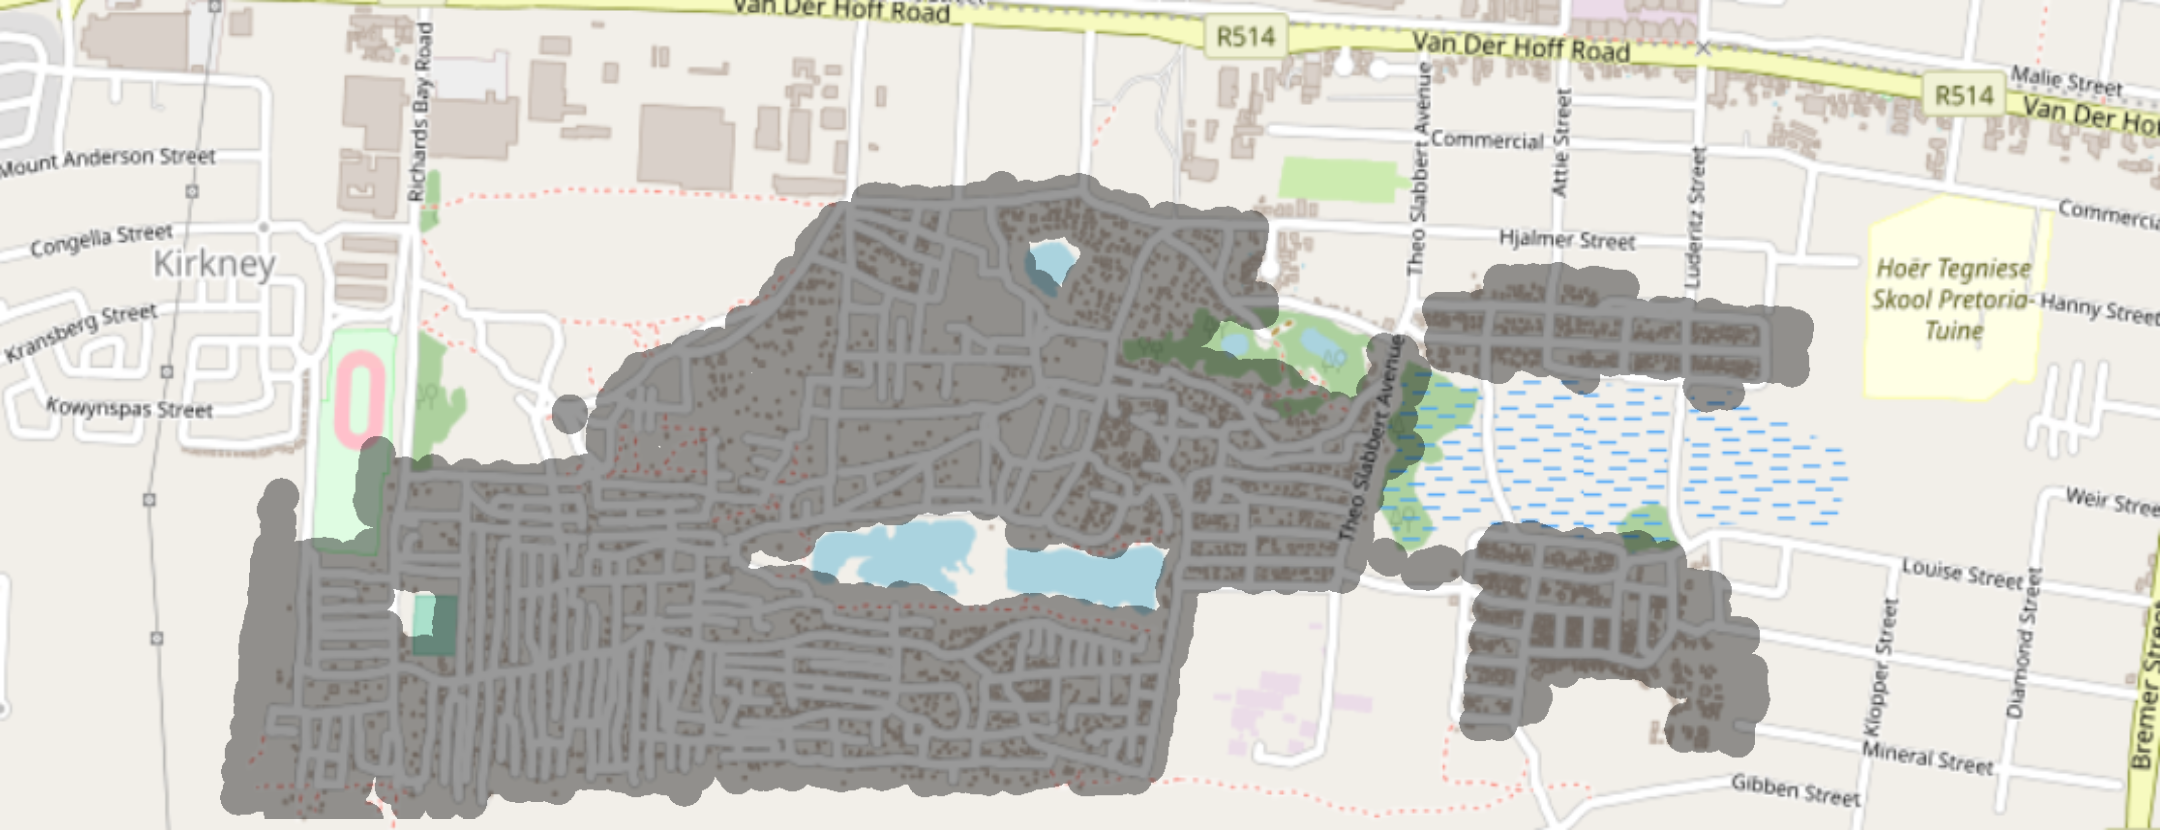
\includegraphics[scale=0.3,angle=90]{Figures/Chapter4/Actual}
\caption{Existing Building Based Land Usage on a Map}
\end{figure}

\begin{figure}[H]
\centering
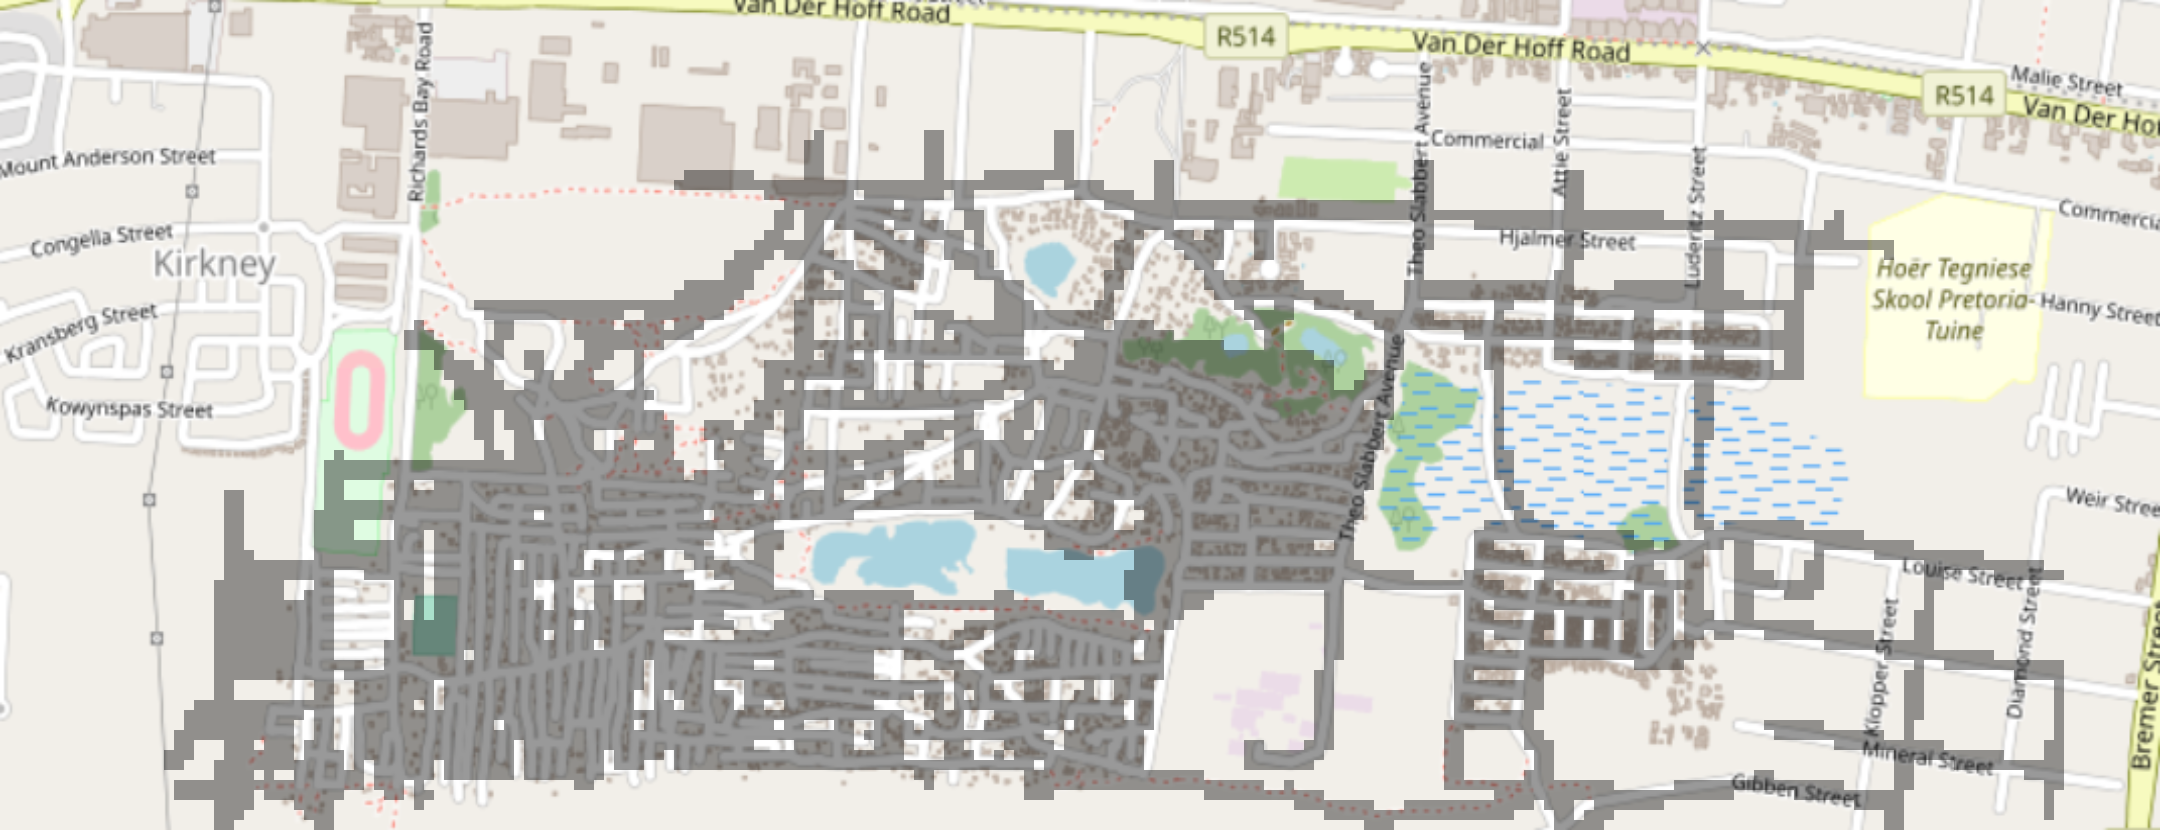
\includegraphics[scale=0.3,angle=90]{Figures/Chapter4/Simulated}
\caption{Simulated Growth of Building Based Land Usage on a Map}
\end{figure}